\documentclass{article}
\usepackage[utf8]{inputenc}
\usepackage{graphicx}
\usepackage{titlepic}
\usepackage{hyperref}
\usepackage{xcolor}
\usepackage{amsmath}


\titlepic{
\includegraphics[width=\textwidth]{pictures/logo.jpg}}
\title{Sending data between Beckhoff PLC and Kuka Robot Controller(KRC4)}
\author{Espen Teigen }
\date{March 2019}




\begin{document}

\maketitle

    Github: https://github.com/EspenTeigen/Kuka-KR-C4-commissioning

\newpage
\section{Setting up the PLC to send and receive data with controller}

\subsection{Opening a project and getting to know the main PLC components}
First you have to open Twincat XAE. you will get this window

\begin{figure}[!h]
    \centering
    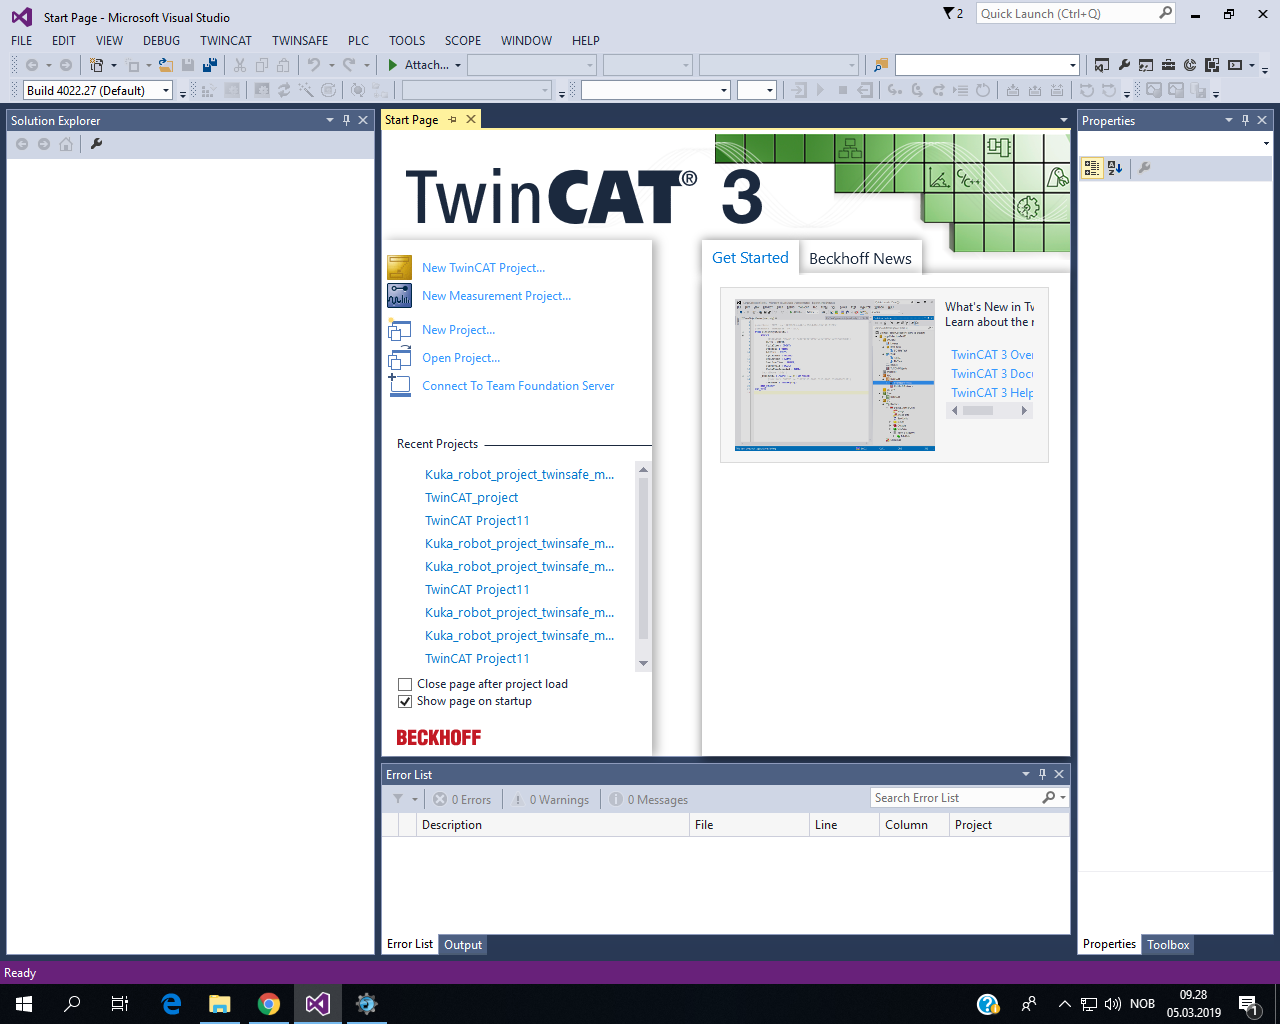
\includegraphics[width=\textwidth]{pictures/TC3_overview/TC3_startscreen.png}
    \caption{Twincat startscreen}
    \label{fig:my_label}
\end{figure}

Select open project and in the folder TwinCAT project, you will find the microsoft visual studio solution \textbf{Kuka\_robot\_project\_twinsafe\_modbus}. If the project is not found, you can get a copy from \href{https://github.com/EspenTeigen/Kuka-KR-C4-commissioning}{\underline{github}}

\newpage
You will get this view

\begin{figure}[!h]
    \centering
    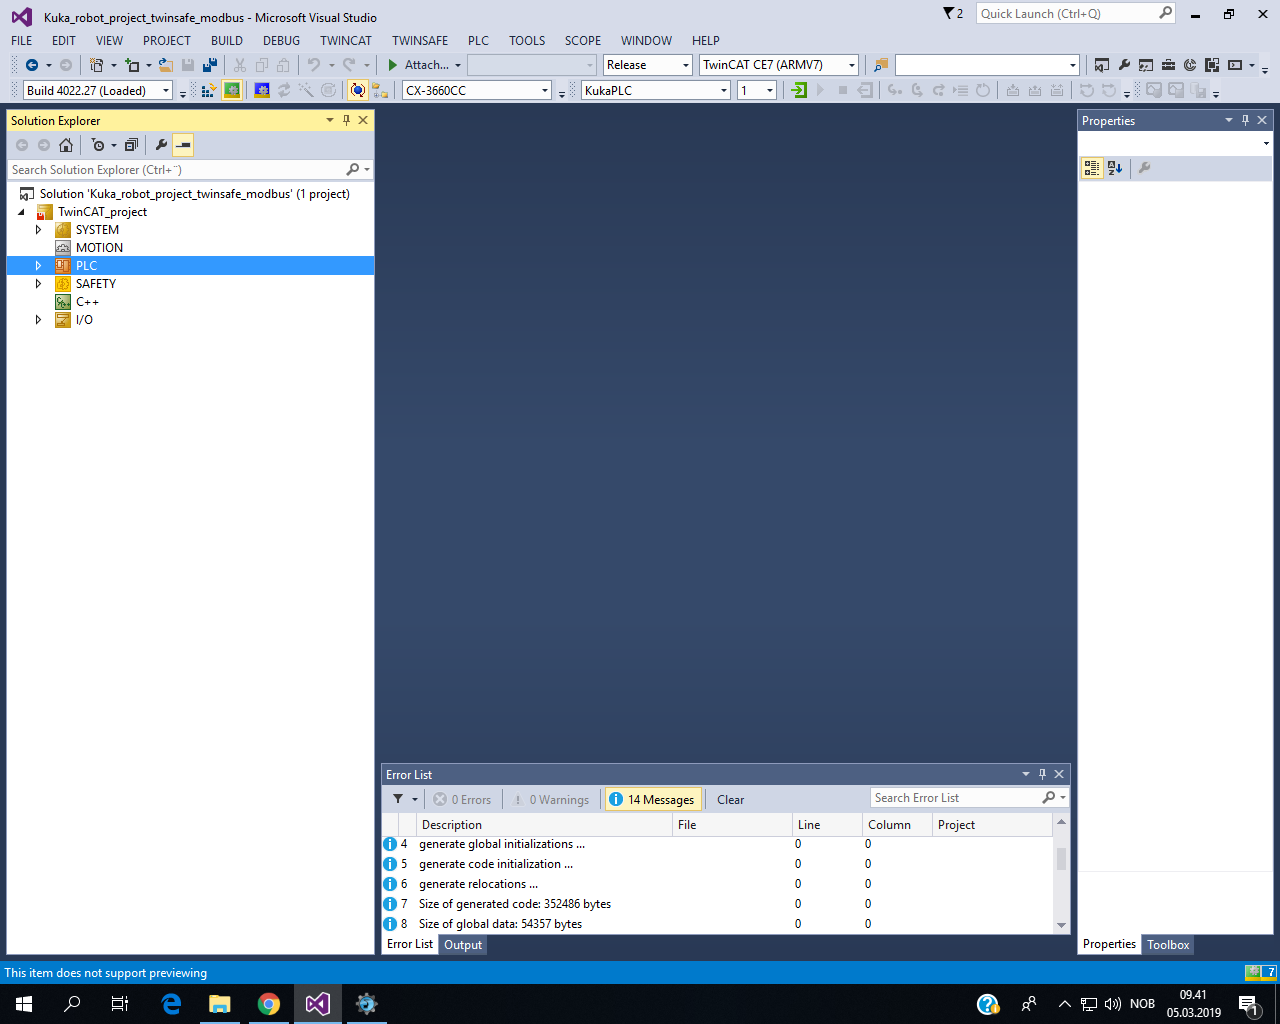
\includegraphics[width=\textwidth]{pictures/TC3_overview/TC3_project_view.png}
    \caption{Project view}
    \label{fig:my_label2}
\end{figure}

The most interesting part off the project tree is the PLC, so expand that part. 
\newpage
We can now take a look at the different parts that are relevant for data transmission.

\begin{figure}[!h]
    \centering
    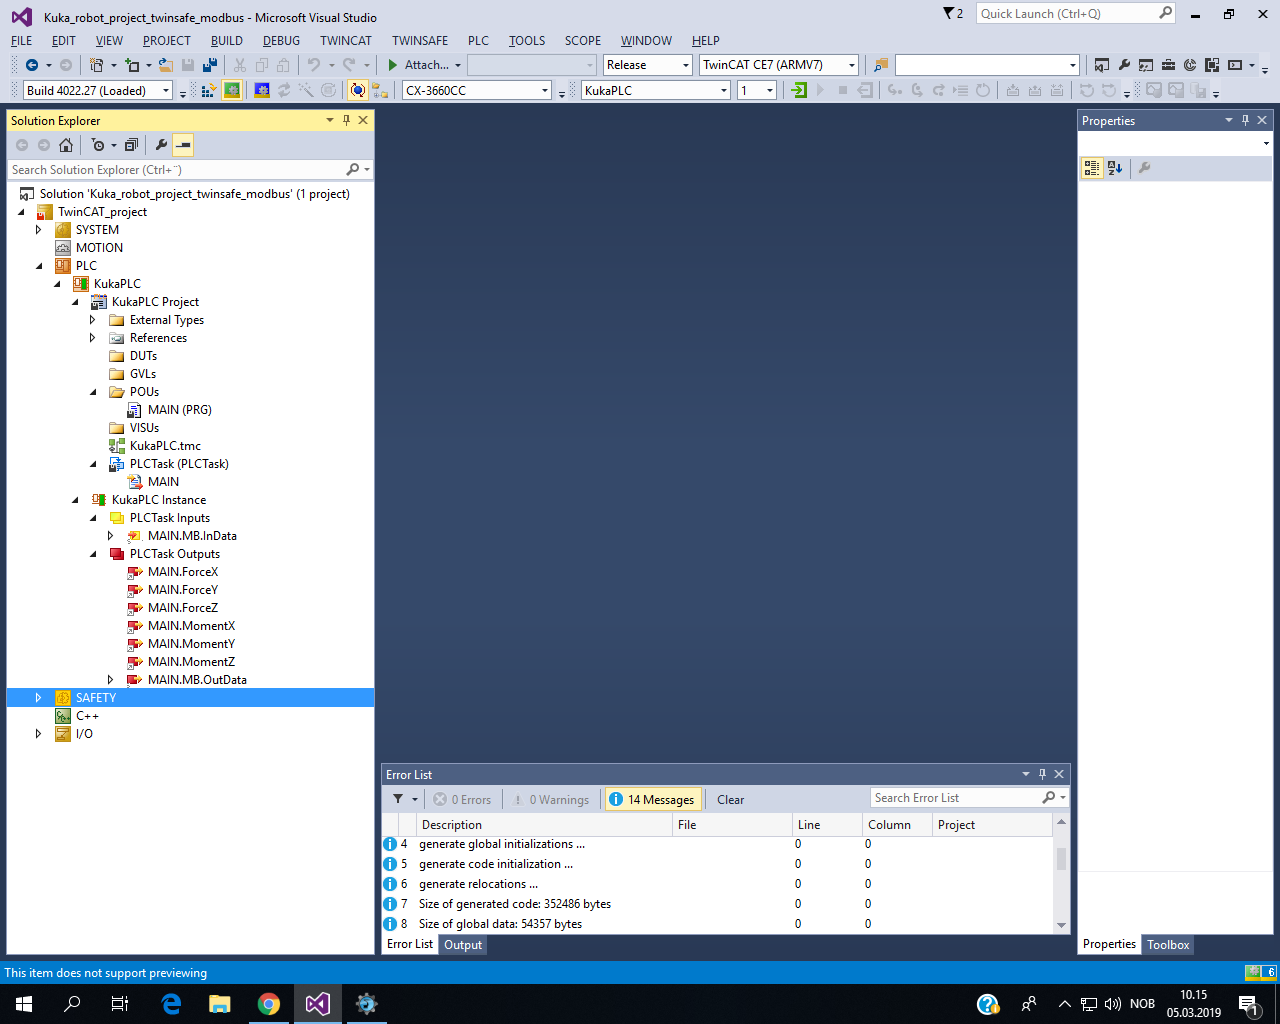
\includegraphics[width=\textwidth]{pictures/TC3_overview/TC3_PLC_expanded.png}
    \caption{Caption}
    \label{fig:my_label}
\end{figure}

\newpage

\subsubsection{KukaPLC Project}
\begin{figure}[!h]
    \centering
    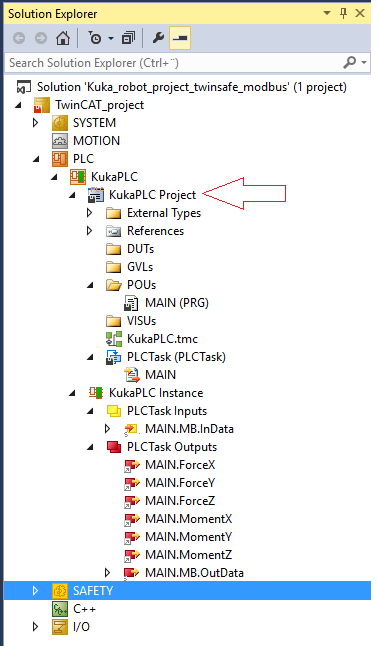
\includegraphics[scale=0.7]{pictures/TC3_overview/TC3_KukaPLC.png}
    \caption{Caption}
    \label{fig:my_label}
\end{figure}
This is the entire PLC project, and are pre-configured to transfer data from the force-torque sensor to the robot controller. It is in this project we will set up our data transfer.  

\newpage

\subsubsection{POUs}
\begin{figure}[!h]
    \centering
    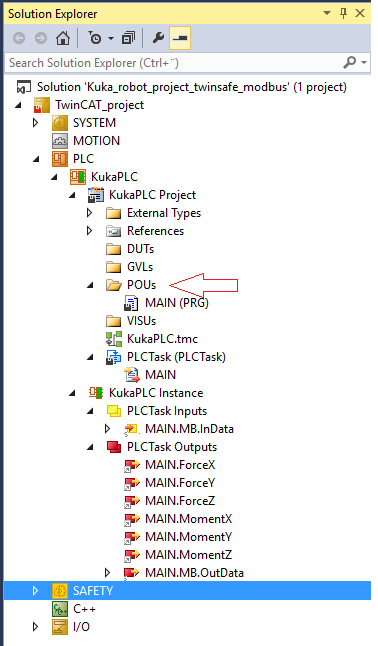
\includegraphics[scale=0.7]{pictures/TC3_overview/TC3_POUs.png}
    \caption{}
    \label{fig:my_label}
\end{figure}

POUs are where at the programs, function blocks and functions are placed. You can chose between all the IEC 61131-3 standard programming languages. I will be using structured text. 

\newpage

\subsubsection{PLCTask}
\begin{figure}[!h]
    \centering
    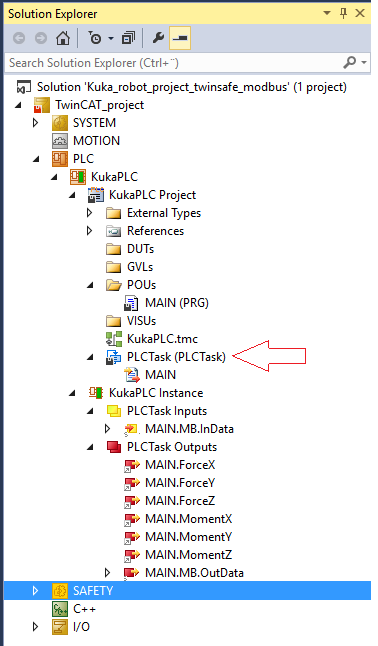
\includegraphics[scale=0.7]{pictures/TC3_overview/TC3_PLCTask.png}
    \caption{}
    \label{fig:my_label}
\end{figure}

To understand this, i have to explain what a task is. A task is controlling the timing of how often the program should be run. You can also configure the priority of how the program should be run. If the program block is of utmost importance, and must be completed within a certain time limit, you will give it a suiting priority. 
\\
\\
PLCtask is a task that I made, and are used for this PLC. Every program that are going to be run in the PLC is timed by this task, and has to be added to it. 


\newpage

\subsubsection{KukaPLC instance}
\begin{figure}[!h]
    \centering
    \includegraphics[scale=0.7]{"pictures/TC3_overview/TC3_KukaPLC Instance".png}
    \caption{}
    \label{fig:my_label}
\end{figure}

This is where you tie you're inputs and outputs to be transferred to and from the robot controller. When you create inputs and outputs in the PLC-program, they will end up here, and you have to link them to the module that transfer the data. Do not fret, I will describe this in a better manner later in the document. 

\newpage

\subsection{Creating a new program}


\begin{figure}[!h]
    \centering
    \includegraphics[scale=0.5]{"pictures/Creating program/create_POU(1)".png}
    \caption{Start by right-clicking on the POUs-folder and select add-POU}
    \label{fig:my_label}
\end{figure}

\begin{figure}[!h]
    \centering
    \includegraphics[scale=0.5]{"pictures/Creating program/POU name(2)".png}
    \caption{Give the program a name, and make sure you create a program, and that it is structured text}
    \label{fig:my_label}
\end{figure}

\newpage

\begin{figure}[!h]
    \centering
    \includegraphics[scale=0.5]{"pictures/Creating program/create IO(3)".png}
    \caption{Now we are ready to write a program}
    \label{fig:my_label}
\end{figure}

\noindent
\textcolor{blue}{PROGRAM}  demonstration is the name of the program
\\\\
\textcolor{blue}{VAR} and \textcolor{blue}{END\_VAR} denotes where you declare variables
\\\\
testVarOutput \textcolor{blue}{AT} \textcolor{purple}{\%Q*} : \textcolor{blue}{DWORD :=} 0;
\\
testVarOutput is the variable name, \textcolor{blue}{AT} tells the compiler that this should be attached to something. \textcolor{purple}{\%Q} tells the compiler that it should be an output, and the asterix * is telling the compiler that it can choose where in memory the data should be saved.    
\\\\
The reason we are using DWORD is because the ethercat bridge is configured to use it. The use of anything else will give a compiler error. 
\\\\
For the variable testVarInput it is the same, except we are using \textcolor{purple}{I} to tell the compiler that it is an input.
\\\\
Lastly I have just written a short code that will iterate trough all the values until the variable overflows and start at zero again. After we have linked the output to the bridge, the value will be transferred to the robot controller every iteration.

\subsection{Connecting the program to the PLC-task}

 Now we have to connect our program to the PLC-task, otherwise it will not be executed. 
 
 \begin{figure}[!h]
     \centering
     \includegraphics[scale=0.5]{"pictures/Creating program/add to task(4)".png}
     \caption{Adding the program to the PLC-task}
     \label{fig:my_label}
 \end{figure}

\begin{figure}[!h]
    \centering
    \includegraphics[scale=0.4]{"pictures/Creating program/select task(5)".png}
    \caption{Select our program to be added to task and click OK}
    \label{fig:my_label}
\end{figure}

\newpage

Ok, just a few more steps. To get our input and output added to the instances, we have to build the PLC-program. 

\begin{figure}[!h]
    \centering
    \includegraphics[scale=0.5]{"pictures/Creating program/build(6)".png}
    \caption{Right click on KukaPLC project and select build}
    \label{fig:my_label}
\end{figure}



\begin{figure}[!h]
    \centering
    \includegraphics[scale=0.5]{"pictures/Creating program/Instance(7)".png}
    \caption{And now we can see the input and output we created in the KukaPLC instance}
    \label{fig:my_label}
\end{figure}

\newpage

\subsection{Linking of variables to bridge}

And to get the data transferred, we have to link this instances to the ethercat-bridge inside the controller. Double-click the demonstration.testVarInput.


\begin{figure}[!h]
    \centering
    \includegraphics[scale=0.5]{"pictures/Creating program/link input(8)".png}
    \caption{We start by linking the input. Click the link to button}
    \label{fig:my_label}
\end{figure}

A new window opens, this shows everything in the system you can link this variable to. If the variable type was BOOL, we could have linked this to a regular input or output. But we are linking this to the ethercat-bridge in the controller. This is the Box 9 (KRC4 secondary EL6695-1001). 

\begin{figure}[!h]
    \centering
    \includegraphics[scale=0.5]{"pictures/Creating program/link input(9)".png}
    \caption{I am choosing the first DWORD, but you could use anyone }
    \label{fig:my_label}
\end{figure}

\newpage

We have successfully(I hope) linked the variable to the ethercat-bridge, and after upload to the PLC we can pull the values from the controller from this variable.
\\\\
Next step is to link the output variable to the ethercat-bridge so we can send values to the robot controller. 
\\\\
Start by double-clicking demonstration.TestVarOut located under PLCTask Outputs and click the Link to button(like you did when linking the input).
\\\\


\begin{figure}[h!]
    \centering
    \includegraphics[scale=0.5]{"pictures/Creating program/link output(11)".png}
    \caption{Since I already have used the six first outputs to the data transfer from the force-torque sensor, we have to select the 6 output.}
    \label{fig:my_label}
\end{figure}

Press OK, and we have also linked our output variable to be sent to the controller. The last step is to download the program to the PLC.

\newpage

\subsection{Downloading the program to the PLC}



\begin{figure}[h!]
    \centering
    \includegraphics[scale=0.8]{"pictures/Creating program/upload(1)".png}
    \caption{Up in the left area of TwinCAT, you can see this button. Push it, just do it, i dare you}
    \label{fig:my_label}
\end{figure}

\begin{figure}[h!]
    \centering
    \includegraphics{"pictures/Creating program/upload(2)".png}
    \caption{Press OK}
    \label{fig:my_label}
\end{figure}

\begin{figure}[h!]
    \centering
    \includegraphics{"pictures/Creating program/upload(3)".png}
    \caption{And press OK again}
    \label{fig:my_label}
\end{figure}

You have now downloaded the program to the PLC, the next step is to configure Work Visual so the controller can receive the values we are sending to it.

\newpage

\section{Configuration of the robot controller to send and receive values to and from the PLC}
So. Lets open Work Visual, and getting started with the configuration to send and receive data. 

\subsection{Getting Work Visual up and running and brief overview}
This is the first window Work Visual greet's you with. 

\begin{figure}[!h]
    \centering
    \includegraphics[scale=0.3]{"pictures/Config work visual/WV(1)".png}
    \caption{Start by clicking browse}
    \label{fig:my_label}
\end{figure}

\newpage

\begin{figure}[!h]
    \centering
    \includegraphics[scale=0.5]{"pictures/Config work visual/WV(2)".png}
    \caption{You are now looking at the files that are on the controller}
    \label{fig:my_label}
\end{figure}

Expand the tree and you will see this

\begin{figure}[!h]
    \centering
    \includegraphics[scale=0.5]{"pictures/Config work visual/WV(3)".png}
    \caption{Notice that the file marked in red has a green arrow. This denotes that it is the active project}
    \label{fig:my_label}
\end{figure}

Click open

\begin{figure}[!h]
    \centering
    \includegraphics[scale=0.5]{"pictures/Config work visual/WV(4)".png}
    \caption{Double-click the project ot make it active}
    \label{fig:my_label}
\end{figure}

\newpage

On the left you will see the project tree for the robot configuration. 

\begin{figure}[!h]
    \centering
    \includegraphics[scale=0.3]{"pictures/Config work visual/WV(5)".png}
    \caption{Expand the Kuka extension bus(SYS-X44)}
    \label{fig:my_label}
\end{figure}



\textcolor{red}{Do not do any configuration with control or system bus if you don't know what you are doing:} This will do major damage to the configuration file, and is thoroughly hard to unfuck. 

\newpage

Lets take a closer look at the project tree

\begin{figure}[!h]
    \centering
    \includegraphics[scale=1]{"pictures/Config work visual/WV(6)".png}
    \caption{\textcolor{red}{1} is the bus our ethercat bridge is connected to, \textcolor{red}{2} is the bus we can connect our IO's and modules to}
    \label{fig:my_label}
\end{figure}

I do not think there should be any need in the near future to do any changes to the settings of the ethercat-bridge. I have configured it to handle 128 bytes of data on each transmission, and 
I think that should be enough for future use. 
\\\\
Now, let's have a look at how we would go about to configure the sending and receiving of data to and from the PLC. 

\newpage

\subsection{Linking the inputs from the PLC}
We are now going to connect the data being sent from the PLC with the controllers internal IO-handling system. 
\\\\
In the center pane, you will find this

\begin{figure}[!h]
    \centering
    \includegraphics[scale=0.7]{"pictures/Config work visual/WV(7)".png}
    \caption{Make sure you are on the IO-maping tab }
    \label{fig:my_label}
\end{figure}
In the left pane, you are looking at the controllers internal IO's. We are going to connect this ones to the IO's comming from the ethercat brdige that are attached to the field-bus. So, in the right pane, select the fieldbusses pane. 

\newpage
Under sys-x44 you will find the EL6695-1001 bridge, select this in the right pane, and inputs ind the left pane.

\begin{figure}[!h]
    \centering
    \includegraphics[scale=0.6]{"pictures/Config work visual/WV(8)".png}
    \caption{We are first adding the values sent from the PLC}
    \label{fig:my_label}
\end{figure}

in this picture, you will see that in the center horizontal pane, there is already some connections. This are the values that are from the force-torque sensor. As mentioned earlier, it is six values, and this matches up with the amount of connections we have. 
\\\\
The bottom right pane is the inputs from the ethercat bridge, and the bottom left, are the inputs on the controller we can connect to. The green arrow denotes the ones that are already connected. 
\\\\
One import thing to know and remember her, is that the controller treats every input as a boolean value, but fortunately, we can put several boolean inputs in to bytes, words and so on.  

\newpage

The data we are receiving are UDINT(Unsigned double integer), and as everyone knows, this is 32 bits. That means that we have to select 32 of the inputs on the bottom left pane to have the space for thr data we are receiving from the PLC. 

\begin{figure}[!h]
    \centering
    \includegraphics[scale=0.6]{"pictures/Config work visual/WV(9)".png}
    \caption{I have expanded the two bottom windows so we can see all the bits i have chosen}
    \label{fig:my_label}
\end{figure}

Notice that in the right window, that i have chosen std.In(128 Bytes.input) DWORD 6. This correlate to where we put the data when we were doing the linking in the PLC.
\newpage
Now we can connect the input to the bits


\begin{figure}[!h]
    \centering
    \includegraphics[scale=0.6]{"pictures/Config work visual/WV(10)".png}
    \caption{By clicking the connect button. Fortunately, I have marked this button with a big red arrow}
    \label{fig:my_label}
\end{figure}



\begin{figure}[!h]
    \centering
    \includegraphics[scale=0.6]{"pictures/Config work visual/WV(11)".png}
    \caption{Click Yes}
    \label{fig:my_label}
\end{figure}

\newpage

We should now have made this connection
\begin{figure}[!h]
    \centering
    \includegraphics[scale=0.6]{"pictures/Config work visual/WV(12)".png}
    \caption{Again we have a big red arrow that show us the change. Take a note of the number to the left, this will be useful later}
    \label{fig:my_label}
\end{figure}

\newpage

\subsection{Linking the outputs to the PLC }

The process of linking the outputs to the PLC is essentially the same, but since I am a nice guy, and I already made the section name  I will walk you trough this too. 
\\\\
Instead of choosing digital input in the upper left pane, we are now going to choose output

\begin{figure}[!h]
    \centering
    \includegraphics[scale=0.7]{"pictures/Config work visual/WV(13)".png}
    \caption{Select the digital output in the left pane, but stay on the EL6695-1001 fieldbus }
    \label{fig:my_label}
\end{figure}

\newpage

The process is going to be the same as last time. In the bottom pane, available outputs are gray, and linked outputs are green. The green one's, are the digital outputs in the cabinet the robot controls. 

\begin{figure}[!h]
    \centering
    \includegraphics[scale=0.7]{"pictures/Config work visual/WV(14)".png}
    \caption{Notice that i made an error, i linked it to output 1 instead. You should use the same as the data you linked in the PLC-program.  }
    \label{fig:my_label}
\end{figure}

Select 32 available outputs and link them to output 0, as we chose in the PLC-program.

\newpage

Push yes on the popup, and it should look something like this.

\begin{figure}[!h]
    \centering
    \includegraphics[scale=0.7]{"pictures/Config work visual/WV(15)".png}
    \caption{Success! Note: The error i made is still there}
    \label{fig:my_label}
\end{figure}

\newpage

\section{Give the output and input usable names}
Since we are nice people, we would like to give the input and output names that we can remember. It can be hard to remember the data value we receive from the PLC is linked to input $n\:to\:n+31$. 

\newline
\newline

\begin{figure}[!h]
    \centering
    \includegraphics[scale=0.6]{"pictures/Config work visual/WV(16)".png}
    \caption{In the bottom left of the screen, click the programming and diagnosis button}
    \label{fig:my_label}
\end{figure}

\newpage

This gives you a new window. This window allows you to navigate the files and folders on the controller. 

\begin{figure}[!h]
    \centering
    \includegraphics[scale=0.5]{"pictures/Config work visual/WV(17)".png}
    \caption{Right click the cookie monster and choose establish controller state to connect to the controller}
    \label{fig:my_label}
\end{figure}

\newpage

Expand R1 and then system, double click config.dat and the center pane will give you a window with som code.

\begin{figure}[!h]
    \centering
    \includegraphics[scale=0.5]{"pictures/Config work visual/WV(18)".png}
    \caption{Double click config.dat and scroll to the bottom}
    \label{fig:my_label}
\end{figure}

Near the bottom you will find User defined externals. This is where we are going to give our input and output a name. And of course some nice comments, so it is easy to understand why they are there. 

\newpage

\begin{figure}[!h]
    \centering
    \includegraphics[scale=0.6]{"pictures/Config work visual/WV(19)".png}
    \caption{I have chosen to use the same variable name as i did on the PLC, but it is not something you must do}
    \label{fig:my_label}
\end{figure}

Congratulations, you have earned a black belt in data transmission between a Beckhoff PLC and Kuka robot controller 4.  

\end{document}
